\documentclass[11pt]{article}

% ---------- Paquetes ----------
\usepackage[utf8]{inputenc}
\usepackage[T1]{fontenc}
\usepackage[margin=2.5cm]{geometry}
\usepackage{amsmath,amssymb}
\usepackage{circuitikz}
\usetikzlibrary{positioning}
\usepackage{enumitem}
\usepackage{booktabs}
\usepackage{array}
\usepackage{tabularx}
\usepackage{graphicx}
\usepackage{xcolor}
\usepackage{titlesec}
\usepackage{hyperref}
\usepackage{fancyhdr}
\usepackage{caption}
\captionsetup{justification=centering, font=it, labelfont={it,bf}}
\captionsetup[figure]{name=Figure}
\captionsetup[table]{name=Table}
\usepackage{float}

\hypersetup{colorlinks=true, linkcolor=blue, urlcolor=blue, citecolor=blue}

\titleformat{\section}{\large\bfseries}{\thesection.}{0.5em}{}
\titleformat{\subsection}{\normalsize\bfseries}{\thesubsection}{0.5em}{}

\pagestyle{fancy}
\fancyhf{}
\fancyhead[L]{Lab. 2 --- Linear Op-Amp Circuits}
\fancyhead[R]{\thepage}
\renewcommand{\headrulewidth}{0.4pt}

\setlength{\parindent}{0pt}
\setlength{\parskip}{0.5em}

\newcommand{\blank}[1]{\makebox[#1]{\hrulefill}}

\begin{document}

% =====================================================
% PORTADA / DATOS DEL EQUIPO
% =====================================================
\begin{center}
    {\LARGE \bfseries Lab. 2}\\[0.3em]
    {\Large \itshape Linear Op-Amp Circuits}
\end{center}

\vspace{1em}

\noindent Team No. 2

\vspace{0.5em}

\noindent Names:


\begin{tabbing}
\hspace{1cm} \= Jefferson Chinchilla Quesada \hspace{0.3cm} \= 2023152266  \\[0.6cm]
\> Mattio Coghi Quirós \> 2023056023 \\[0.6cm]
\> Nicolás Mena Valerio \> 2022327473
\end{tabbing}

\vspace{1em}
\vspace{1em}

% =====================================================
% REFERENCIA Y LECTURA
% =====================================================
\subsection*{Reference:}
Floyd Thomas L., Buchla David M.: \textit{Experiments in Analog Fundamentals, A System Approach}. Pearson Education, 2013.

\subsection*{Reading:}
Floyd and Buchla, \textit{Fundamentals: A Systems Approach}, Sections 6-4 through 6-6. Pearson Education, 2013.

\subsection*{Objectives:}
After performing this experiment, you will be able to:
\begin{enumerate}[label=\arabic*.]
    \item Construct and test inverting and noninverting amplifiers using op-amps.
    \item Specify components for inverting and noninverting amplifiers using op-amps.
\end{enumerate}

\subsection*{Materials Needed:}
\begin{itemize}
    \item Resistors: two $1\,\text{k}\Omega$, one $10\,\text{k}\Omega$, one $470\,\text{k}\Omega$, one $1.0\,\text{M}\Omega$
    \item Two $1.0\,\mu\text{F}$ capacitors
    \item One 741C op-amp
    \item \textit{For Further Investigation:}
    \begin{itemize}
        \item One $1.0\,\text{k}\Omega$ potentiometer, one $100\,\text{k}\Omega$ resistor, assorted resistors to test.
    \end{itemize}
\end{itemize}

% =====================================================
% SUMMARY OF THEORY
% =====================================================
\section*{Summary of Theory}

One of the most important ideas in electronics incorporates the idea of \textit{feedback}, where a portion of the output is returned to the input. If the return signal tends to decrease the input amplitude, it is called \textit{negative feedback}. Negative feedback produces a number of desirable qualities in an amplifier, increasing its stability and its frequency response. It also allows the gain to be controlled independently of the device parameters, temperature, or other variables.

Operational amplifiers are almost always used with external, negative feedback. The feedback circuit determines the specific characteristics of the amplifier. By itself, an op-amp has an extremely high voltage gain called the \textit{open-loop} gain, $A_{ol}$. When negative feedback is added, the overall gain of the amplifier is determined by the feedback circuit. This gain, including the feedback circuit, is called the \textit{closed-loop} gain, $A_{cl}$.

Figure~\ref{fig:20-1} illustrates a noninverting amplifier with negative feedback. The input is applied to the noninverting terminal and a fraction ($B$) of the output is returned to the inverting input by the voltage divider. The very high gain of the amplifier forces the two inputs to be very nearly the same voltage; therefore, the input voltage is across $R_i$, and the output voltage is across $R_i + R_f$. The closed-loop gain of this noninverting amplifier is given as $A_{cl(NI)}$. The closed-loop gain is the reciprocal of the feedback fraction, as shown in Figure~\ref{fig:20-1}.

\begin{figure}[h!]
\centering
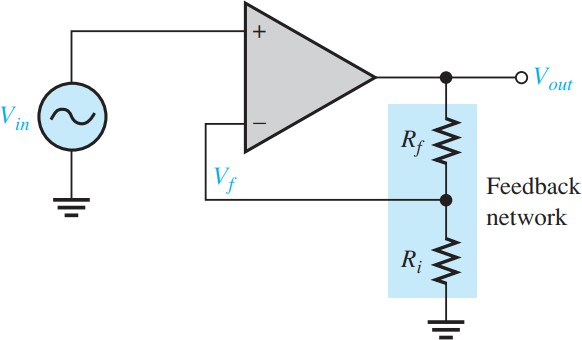
\includegraphics[width=0.6\textwidth]{figs/image1.jpeg}
\caption{Noninverting amplifier}
\label{fig:20-1}
\end{figure}

\begin{align*}
\text{feedback fraction} = B = \dfrac{R_i}{R_i + R_f}
\end{align*}

\begin{align*}
A_{cl(NI)} = \dfrac{1}{B} = \dfrac{R_i + R_f}{R_i} = 1 + \dfrac{R_f}{R_i}
\end{align*}

An inverting amplifier is shown in Figure~\ref{fig:20-2}. In this amplifier, the output voltage is the opposite phase to the input voltage. The noninverting input is grounded, and the input signal is applied through a resistor to the inverting terminal. A feedback resistor is connected between the output and the inverting input. This amplifier can be analyzed by assuming the input current is the same as the current in the feedback resistor, $I_{in} = I_f$, and that the open-loop gain of the amplifier is very high. From these assumptions, the closed-loop gain can be calculated quite accurately as the ratio of the feedback resistor to the input resistor. The basic equations for the inverting amplifier are shown with Figure~\ref{fig:20-2}. The minus sign indicates inversion between the input and output. $(-)$ refers to the inverting input on the op-amp.

\begin{figure}[h!]
\centering
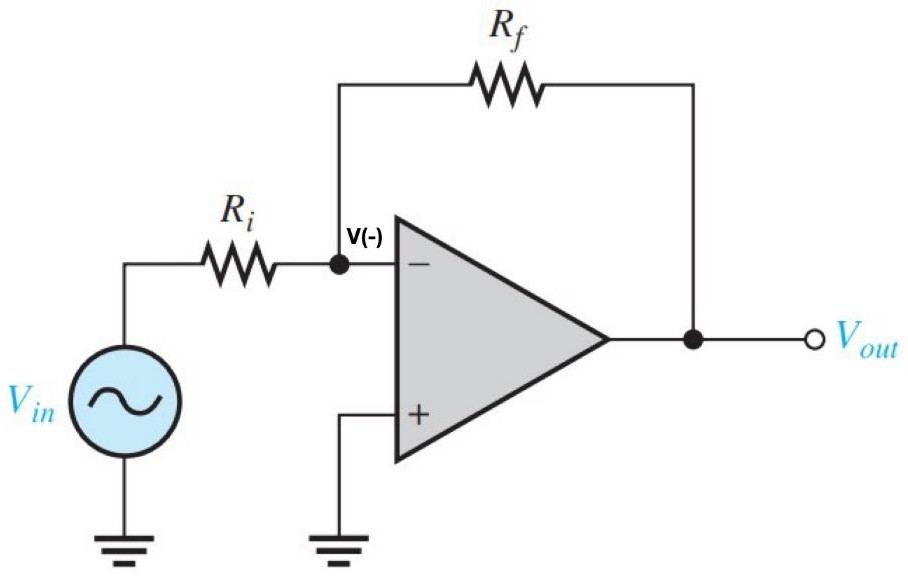
\includegraphics[width=0.65\textwidth]{figs/image2.jpeg}
\caption{Inverting amplifier}
\label{fig:20-2}
\end{figure}

\begin{align*}
I_{in} = I_f
\end{align*}

$A_{ol}$ is very large, therefore
\begin{align*}
V(-) = -\dfrac{V_{out}}{A_{ol}} \cong 0
\end{align*}

\begin{align*}
\dfrac{V_{in}}{R_i} = -\dfrac{V_{out}}{R_f}
\end{align*}

\begin{align*}
A_{cl(I)} = \dfrac{V_{out}}{V_{in}} = -\dfrac{R_f}{R_i}
\end{align*}

\newpage
% =====================================================
% PROCEDURE
% =====================================================
\section*{Procedure}

\begin{enumerate}[label=\arabic*.]
    \item The circuit to be tested in this step is the noninverting amplifier illustrated in Figure~\ref{fig:20-3}.
    \begin{enumerate}[label=\alph*.]
        \item Measure a $10\,\text{k}\Omega$ resistor for $R_f$ and $1.0\,\text{k}\Omega$ resistor for $R_i$. Record the measured value of resistance in Table~\ref{tab:20-1}.
        \item Using the measured resistances, compute the closed-loop gain of the noninverting amplifier. The closed-loop gain equation is given next to Figure~\ref{fig:20-1}.
        \item Calculate $V_{out}$ using the computed closed-loop gain.
        \item Connect the circuit shown in Figure~\ref{fig:20-3}. Set the signal generator for a $500\,\text{mV}_{pp}$ sinusoidal wave at $1.0\,\text{kHz}$. The generator should have no dc offset.
        \item Measure the output voltage, $V_{out}$. Record the measured value.
        \item Measure the feedback voltage at pin 2. Record the measured value.
        \item Place a $1.0\,\text{M}\Omega$ test resistor in series with the generator. Measure the input resistance of the circuit, $R_{in}$, based on the voltage drop across the test resistor. Use the voltage divider rule to indirectly find the input resistance.
    \end{enumerate}
\end{enumerate}

\begin{table}[h!]
\centering
\caption{Noninverting amplifier measurements}
\label{tab:20-1}
\resizebox{\textwidth}{!}{%
\begin{tabular}{|c|c|c|c|c|c|c|c|}
\hline
$R_f$ & $R_i$ & $V_{in}$ & $A_{cl(NI)}$ & $V_{out}$ & $V_{out}$ & $V(-)$ & $R_{in}$ \\
Measured & Measured & Measured & Computed & Computed (pin 6) & Measured (pin 6) & Measured (pin 2) & Measured \\
\hline
 $10$ k$\Omega$& $1$ k$\Omega$ & $500\,\text{mV}_{pp}$ & $11$ & $5.5$ Vpp & $5.56$ Vpp & $556$ mV  & $654$ k$\Omega$ \\[1.2em]
\hline
\end{tabular}%
}	
\end{table}

\begin{figure}[h!]
\centering
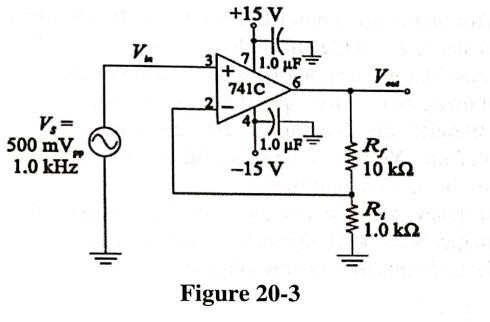
\includegraphics[width=0.55\textwidth]{figs/fig20-3.jpeg}
\caption{Noninverting amplifier test circuit (741C, $R_f = 10\,\text{k}\Omega$, $R_i = 1.0\,\text{k}\Omega$)}
\label{fig:20-3}
\end{figure}

El $R_{in}$ de la tabla se obtiene con la regla del divisor de tensión. El generador de $500\,\text{mV}_{pp}$ equivale a $176.8\,\text{mV}_{rms}$ y en la entrada del amplificador se midieron $69.91\,\text{mV}_{rms}$, así que sobre el resistor de prueba de $1.0\,\text{M}\Omega$ caen los $106.87\,\text{mV}_{rms}$ restantes.

\begin{align*}
R_{in} = R_{prueba}\,\frac{V_{R_{in}}}{V_s - V_{R_{in}}} = 1\,\text{M}\Omega \cdot \frac{69.91\,\text{mV}}{106.87\,\text{mV}} = 654\,\text{k}\Omega
\end{align*}

Este valor queda muy por debajo de lo que predice la teoría, porque la realimentación negativa multiplica la resistencia de entrada del 741C por $(1 + A_{ol}B)$ y la lleva al orden de los $\text{G}\Omega$. Lo que limita la medición es la carga del instrumento, la punta del osciloscopio y el camino de corriente de polarización quedan en paralelo con la entrada y son del orden de los $\text{M}\Omega$, de modo que el divisor termina midiendo esa combinación.


Como demuestra la señal de salida $V_{out}$ en la figura \ref{fig:fig1} se observa el efecto de amplificación $Av$ = 11.

\begin{figure} [H]
	\centering
	
\includegraphics[width=0.7\linewidth]{figs/DS0001}
	\caption{Señal de salida $V_{out}$ amplificada}
	\label{fig:fig1}
\end{figure}


\newpage

\begin{enumerate}[resume, label=\arabic*.]
    \item In this step you will test an inverting amplifier. All data are to be recorded in Table~\ref{tab:20-2}. The circuit is illustrated in Figure~\ref{fig:20-4}. The closed-loop gain is:
    \begin{align*}
    A_{cl(I)} = -\dfrac{R_f}{R_i}
    \end{align*}
    \begin{enumerate}[label=\alph*.]
        \item Use the same resistors for $R_f$ and $R_i$ as in step 1. Record the measured value of resistance in Table~\ref{tab:20-2}.
        \item Using the measured resistance, compute and record the closed-loop gain of the inverting amplifier.
        \item Calculate the $V_{out}$ using the computed closed-loop gain.
        \item Connect the circuit shown in Figure~\ref{fig:20-4}. Set the signal generator for the $500\,\text{mV}_{pp}$ sine wave at $1\,\text{kHz}$. The generator should have no dc offset.
        \item Measure and record the output voltage, $V_{out}$.
        \item Measure and record the output voltage at pin 2. This point is called a \textit{virtual ground} because of the effect of negative feedback.
        \item Place a $1.0\,\text{k}\Omega$ test resistor in series with the generator and $R_i$. Measure the input resistance of the circuit, $R_{in}$, based on the voltage drop across the test resistor. In this case, you should observe that the drop across the test resistor is about the same as the drop across $R_i$.
    \end{enumerate}
\end{enumerate}

\begin{table}[h!]
\centering
\caption{Inverting amplifier measurements}
\label{tab:20-2}
\resizebox{\textwidth}{!}{%
\begin{tabular}{|c|c|c|c|c|c|c|c|}
\hline
$R_f$ & $R_i$ & $V_{in}$ & $A_{cl(NI)}$ & $V_{out}$ & $V_{out}$ & $V(-)$ & $R_{in}$ \\
Measured & Measured & Measured & Computed & Computed (pin 6) & Measured (pin 6) & Measured (pin 2) & Measured \\
\hline
 10 \text{ k}$\Omega$ & $1\text{ k}\Omega$ & $50\,\text{mV}_{pp}$ & $-10$ & $5$ V & $4.48$ V & $4.39$ mV & $976\ \Omega$ \\[1.2em]
\hline
\end{tabular}%
}
\end{table}

\begin{figure}[h!]
\centering
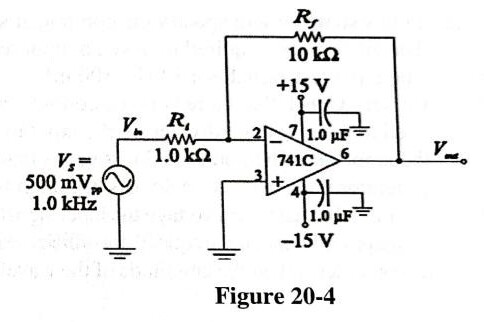
\includegraphics[width=0.55\textwidth]{figs/fig20-4.jpeg}
\caption{Inverting amplifier test circuit (741C, $R_f = 10\,\text{k}\Omega$, $R_i = 1.0\,\text{k}\Omega$)}
\label{fig:20-4}
\end{figure}

Acá el resistor de prueba es de $1.0\,\text{k}\Omega$ y el nodo de entrada quedó en $87.29\,\text{mV}_{rms}$, prácticamente la mitad de los $176.8\,\text{mV}_{rms}$ del generador, tal como anticipa el enunciado.

\begin{align*}
R_{in} = 1\,\text{k}\Omega \cdot \frac{87.29\,\text{mV}}{176.78\,\text{mV} - 87.29\,\text{mV}} = 976\,\Omega
\end{align*}

El resultado cae a un $1.4\,\%$ del $R_i$ medido de $0.9897\,\text{k}\Omega$. Tiene sentido, en el amplificador inversor la señal entra por $R_i$ contra la tierra virtual del pin 2, así que la resistencia de entrada del circuito queda fijada por ese resistor.

En la figura \ref{fig:fig2} se observa la señal de salida $V_{out}$ en modo de retroalimentación negativa, donde se ve claramente que la amplificación respeta la relación $R_f / R_i$, que al ser iguales da un valor de 1. 

\begin{figure} [H]
	\centering
	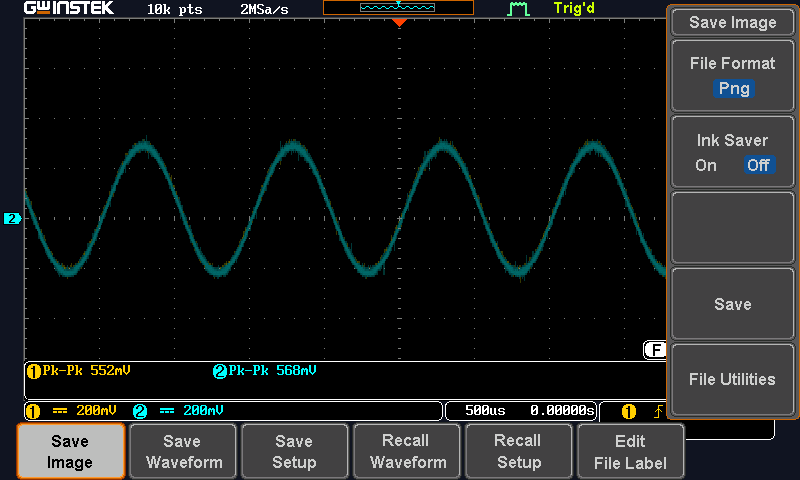
\includegraphics[width=0.7\linewidth]{figs/DS0002}
	\caption{Señal de salida $V_{out}$}
	\label{fig:fig2}
\end{figure}


\newpage

\begin{enumerate}[resume, label=\arabic*.]
    \item In this step you will specify the components for an inverting amplifier using a 741C Op-Amp. The amplifier is required to have an input resistance of $10\,\text{k}\Omega$ and a closed-loop gain of $-47$. The input test signal is a $1\,\text{kHz}$, $100\,\text{mV}_{pp}$ sinusoidal wave signal with no dc component (offset). Check that there is no dc component using an oscilloscope. If necessary, you may need to put a voltage divider on the input to attenuate the signal to the $100\,\text{mV}$ level.

    Draw the amplifier. Then build and test your circuit.

    \textit{Note}: You need to be careful that the generator does not have a dc offset: remember this is a dc amplifier!

    Find the maximum voltage the input signal can have before clipping occurs. Try increasing the frequency and note the frequency at which the output is distorted. Does the upper frequency response depend on the amplitude of the waveform? Summarize your results in the space provided.
\end{enumerate}

A continuación se detalla el proceso de simulación de esta sección:

Primero se calcula el valor de $R_f$ mediante una simple ecuación:

\begin{align*}
	A_{cl} &= - \frac{R_f}{R_i}\\
	47 &=  \frac{R_f}{10 \text{ k}\Omega}\\
	R_f &=  470\text{ k}\Omega\\
\end{align*}

Ahora para calcular en que punto el amplificador se satura basta con hacer la siguiente ecuación:
\begin{align*}
	&15\text{ V} = -47 \cdot V_{in_{max}}\\
	&V_{in_{max}} = 320\text{ mV}\\
\end{align*}

Este comportamiento se evidencia en las siguientes capturas:

\begin{figure} [h!]
	\centering
	\includegraphics[width=0.7\linewidth]{"figs/Captura desde 2026-08-30 21-28-20"}
	\caption{Vin de $100$ mVpp }
	\label{fig:captura-desde-2026-08-30-21-28-20}
\end{figure}


\begin{figure} [h!]
	\centering
	\includegraphics[width=0.7\linewidth]{"figs/Captura desde 2026-08-30 21-35-48"}
	\caption{Vin de $300$ mVpp}
	\label{fig:captura-desde-2026-08-30-21-35-48}
\end{figure}

\begin{figure} [h!]
	\centering
	\includegraphics[width=0.7\linewidth]{"figs/Captura desde 2026-08-30 21-36-46"}
	\caption{Vin de $640$ mVpp}
	\label{fig:64mvpp}
\end{figure}

En la figura \ref{fig:64mvpp} se observa como la señal de salida se empieza a recortar, ya que supera los $15$ V.

\newpage
En cuanto a las simulaciones de respuesta en frecuencia se utilizó un barrido AC para comprobar el comportamiento del circuito a medida que se aumentaba la frecuencia de la señal de entrega. El resultado de esta simulación se muestra en la figura \ref{fig:Respuesta_frecuencia}.

\begin{figure} [H]
	\centering
	\includegraphics[width=0.8\linewidth]{"figs/Captura desde 2026-08-30 22-03-24"}
	\caption{Respuesta en frecuencia del amplificador Inversor}
	\label{fig:Respuesta_frecuencia}
\end{figure}

En dicha imagen se observa el punto exacto en donde el circuito deja de realizar su función de amplificación, mostrando claramente la frecuencia de corte ($f_c = 21\text{ kHz}$). Sin embargo, la señal no se distorsiona con la frecuencia, sino que se atenuá. 
Para determinar la dependencia de la frecuencia y la magnitud, se probaron valores de $V_{in}$ y $f$ hasta alcanzar una distorsión. En este caso se logro al aumentar la tensión a $600$ mVp y con una frecuencia de $40$ kHz, este resultado se observa en la figura \ref{fig:distorsionmagfrecuencia}.\\

Por otro lado, en la medición de laboratorio se demostró que la distorsión ocurrió con una tensión de  $600$ mVp y una frecuencia de $60$ Khz como lo muestra la imagen \ref{fig:distor}

%Insertar imagen del osciloscopio

\begin{figure} [H]
	\centering
	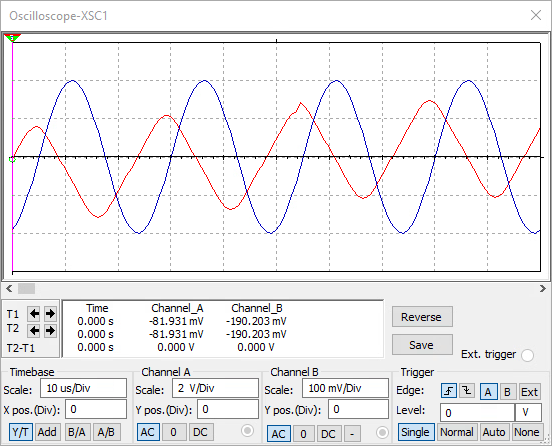
\includegraphics[width=0.7\linewidth]{figs/distorsion_mag_frecuencia}
	\caption{Distorsión de la señal}
	\label{fig:distorsionmagfrecuencia}
\end{figure}

\begin{figure} [H]
	\centering
	
\includegraphics[width=0.7\linewidth]{figs/DS0004}
	\caption{Distorsión de la señal}
	\label{fig:distor}
\end{figure}


\vspace{6cm}

\newpage
% =====================================================
% CONCLUSION
% =====================================================
\section*{Conclusion}

De acuerdo con los circuitos simulados y probados en laboratorio, se confirma la estrecha relación entre la teoría y la práctica en el uso de amplificadores operacionales en configuraciones inversora y no inversora. Se logró observar el efecto de amplificación en la señal de salida, el cual responde directamente a la relación de las resistencias y a la topología elegida para la entrada de tensión. A su vez, se comprobó el comportamiento de las resistencias de entrada ($R_{in}$) en ambos circuitos: en el inversor esta depende del valor de $R_i$, mientras que en el no inversor es teóricamente muy alta, aunque en la práctica se vio limitada por el efecto de carga de los instrumentos de medición.

Por otro lado, al evaluar los límites del OPAMP 741C, se documentó cómo la señal de salida se recorta al alcanzar los voltajes de saturación de la fuente. Además, al superar la frecuencia de corte (aproximadamente a los 21 kHz) y al combinar el aumento de frecuencia con un aumento en la amplitud de la señal de entrada, la onda se atenúa y se deforma, adquiriendo una forma triangular con cierto nivel de offset. Finalmente, la aplicación del OPAMP como óhmetro demostró la alta sensibilidad del circuito, donde la precisión de los componentes (como el potenciómetro) es crítica para lograr una calibración correcta y evitar márgenes de error elevados.

\vspace{9cm}

\newpage
% =====================================================
% EVALUATION AND REVIEW QUESTIONS
% =====================================================
\section*{Evaluation and Review Questions}

\begin{enumerate}[label=\arabic*.]
    \item Express the gain of the amplifiers tested in steps 1 and 2 in dB.
    
    \[A_{cl(NI)} = 20 log(11) = 20.8\text{ dB}\]
    \[A_{cl(I)} = 20 log(10)  = 20\text{ dB}\]

    \vspace{2.5cm}

    \item It was correct to talk about a virtual ground for the inverting amplifier. Why isn't it correct to refer to a virtual ground for the noninverting amplifier?
    
    Debido a la configuración de No inversor la terminal negativa no está conectada a tierra.

    \vspace{2.5cm}

    \item If $R_f = R_i = 10\,\text{k}\Omega$, what gain would you expect for:
    \begin{enumerate}[label=\alph*.]
        \item A noninverting amplifier?
        \[A_{cl(NI)}= 1 + \frac{10 \text{ k}\Omega}{10 \text{ k}\Omega} = 2\]
        \item An inverting amplifier?
        \[A_{cl(I)}= \frac{-R_f}{R_i} = -1\]
    \end{enumerate}

    \vspace{2.5cm}

    \item For the noninverting amplifier in Figure 20-3:
    \begin{enumerate}[label=\alph*.]
        \item If $R_f = 0$ and $R_i$ is infinite, what is the gain?\\
        Si se realizan dichos cambios, la ganancia sería 1.
        \[A_{cl(NI)} = 1 + \frac{0}{\infty} = 1\]

        \vspace{1cm}

        \item What is this type of amplifier called?\\
        Corresponde a un seguidor de voltaje.
    \end{enumerate}

    \vspace{2cm}

    \item What output would you expect in the inverting amplifier of Figure 20-4 if $R_f$ were open?\\
    La salida se recortaría, ya que la señal se amplificaría en un factor de $A_{ol}$ el cual suele ser muy alto, provocando que el amplificador se sature. La señal de salida se vería con varios recorte en los picos y valles, pareciendo una onda cuadrada.

    \vspace{2.5cm}
\end{enumerate}

\newpage
% =====================================================
% FOR FURTHER INVESTIGATION
% =====================================================
\section*{For Further Investigation}

An interesting application of an inverting amplifier is to use it as the basis of an ohmmeter for high value resistors. The circuit is shown in Figure~\ref{fig:20-5}. The unknown resistor, labeled $R_x$, is placed between the terminals. The output voltage is proportional to the unknown resistance.

Calibrate the meter by placing a known $10\,\text{k}\Omega$ resistor in place of $R_x$ and adjusting the potentiometer for exactly $100\,\text{mV}$ output. The output then represents $10\,\text{mV}/1000\,\Omega$. By reading the output voltage, and moving the decimal point, you can directly read resistors from several thousand ohms to over $1\,\text{M}\Omega$.

Construct the circuit and test it using different resistors. Calibrate output voltage against resistance and compare with theory. Find the percent error for a $1\,\text{M}\Omega$ resistor using a lab meter as a standard.

Summarize your results in a short report.

\begin{figure}[h!]
\centering
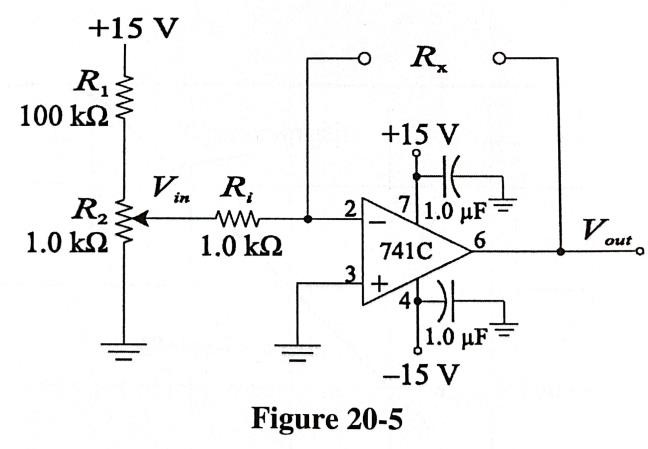
\includegraphics[width=0.5\textwidth]{figs/image4.jpeg}
\caption{Ohmmeter circuit based on the inverting amplifier}
\label{fig:20-5}
\end{figure}

A continuación se resumen los resultados de esta sección.

Con la calibración que pide el enunciado, $100\,\text{mV}$ de salida para un $R_x$ conocido de $10\,\text{k}\Omega$, la escala del óhmetro queda en $10\,\text{mV}$ por cada $1000\,\Omega$. Bajo esa escala un resistor de $1\,\text{M}\Omega$ tendría que dar $10\,\text{V}$ a la salida.

El resistor bajo prueba se midió primero con el multímetro de laboratorio, que se toma como patrón, y dio $R_x = 0.9959\,\text{M}\Omega$. Con ese mismo resistor conectado entre las terminales, la salida del circuito fue de $V_{out} = 14.63\,\text{V}$, que llevada a resistencia con la escala calibrada equivale a una lectura de $1.463\,\text{M}\Omega$.

\begin{align*}
\%\,\text{error} &= \frac{1.463\,\text{M}\Omega - 0.9959\,\text{M}\Omega}{0.9959\,\text{M}\Omega} \times 100\\
\%\,\text{error} &= 46.9\,\%
\end{align*}

El error es grande y además es un factor casi constante, la lectura sale $1.469$ veces el valor patrón. El origen está en la calibración, ya que el montaje se hizo con un potenciómetro de $10\,\text{k}\Omega$ y el enunciado pide uno de $1.0\,\text{k}\Omega$. Devolviendo la cuenta desde la salida medida se obtiene la tensión de entrada con la que realmente se trabajó.

\begin{align*}
V_{in} = \frac{V_{out}\,R_i}{R_x} = \frac{14.63\,\text{V} \times 1\,\text{k}\Omega}{995.9\,\text{k}\Omega} = 14.69\,\text{mV}
\end{align*}

Son $14.69\,\text{mV}$ en lugar de los $10\,\text{mV}$ que corresponden a la escala de $10\,\text{mV}/1000\,\Omega$, y esa razón de $1.469$ es justo el $46.9\,\%$ de error que dio la lectura. El potenciómetro más grande hace muy difícil acertarle al punto de ajuste. Con el de $1.0\,\text{k}\Omega$ la tensión de entrada recorre de $0$ a $148\,\text{mV}$ y los $10\,\text{mV}$ de la calibración caen cerca del $7\,\%$ del recorrido del cursor, mientras que con el de $10\,\text{k}\Omega$ el rango sube hasta $1.36\,\text{V}$ y esos mismos $10\,\text{mV}$ quedan por debajo del $1\,\%$, donde un movimiento mínimo corre toda la escala.

Vale agregar que a $14.63\,\text{V}$ la salida ya queda cerca del límite de excursión del 741C, así que con esa calibración un resistor apenas mayor se habría recortado. Repitiendo la medición con el potenciómetro de $1.0\,\text{k}\Omega$, la lectura para este $R_x$ tendría que quedar alrededor de los $9.96\,\text{V}$ esperados.

\end{document}
